\RequirePackage[T1]{fontenc}
\documentclass[conference]{IEEEtran}
\usepackage{amsmath,amssymb,graphicx,booktabs,url}
\setcounter{dbltopnumber}{3}
\renewcommand{\dbltopfraction}{0.85}
\renewcommand{\textfraction}{0.1}
\renewcommand{\topfraction}{0.9}
\setcounter{topnumber}{3}
\usepackage[hidelinks]{hyperref}
\newcommand{\val}[1]{\csname S#1\endcsname}
\expandafter\def\csname SB2street90\endcsname{3.062}
\expandafter\def\csname SB2street180\endcsname{3.029}
\expandafter\def\csname SB2clean\endcsname{C180}
\expandafter\def\csname SB2accepted\endcsname{0}
\expandafter\def\csname SB2qualified\endcsname{N}
\expandafter\def\csname SB3street90\endcsname{2.766}
\expandafter\def\csname SB3street180\endcsname{2.244}
\expandafter\def\csname SB3clean\endcsname{0}
\expandafter\def\csname SB3accepted\endcsname{270}
\expandafter\def\csname SB3qualified\endcsname{Y}
\expandafter\def\csname SB4street90\endcsname{2.766}
\expandafter\def\csname SB4street180\endcsname{2.244}
\expandafter\def\csname SB4clean\endcsname{0}
\expandafter\def\csname SB4accepted\endcsname{270}
\expandafter\def\csname SB4qualified\endcsname{Y}
\expandafter\def\csname SB5street90\endcsname{2.760}
\expandafter\def\csname SB5street180\endcsname{2.241}
\expandafter\def\csname SB5clean\endcsname{0}
\expandafter\def\csname SB5accepted\endcsname{270}
\expandafter\def\csname SB5qualified\endcsname{Y}
\expandafter\def\csname SB6street90\endcsname{2.650}
\expandafter\def\csname SB6street180\endcsname{2.172}
\expandafter\def\csname SB6clean\endcsname{2}
\expandafter\def\csname SB6accepted\endcsname{264}
\expandafter\def\csname SB6qualified\endcsname{Y}
\expandafter\def\csname SNIS0street90\endcsname{2.647}
\expandafter\def\csname SNIS0street180\endcsname{2.171}
\expandafter\def\csname SNIS0clean\endcsname{0}
\expandafter\def\csname SNIS0accepted\endcsname{254}
\expandafter\def\csname SNIS0qualified\endcsname{Y}
\expandafter\def\csname SNIS1street90\endcsname{2.766}
\expandafter\def\csname SNIS1street180\endcsname{2.244}
\expandafter\def\csname SNIS1clean\endcsname{0}
\expandafter\def\csname SNIS1accepted\endcsname{270}
\expandafter\def\csname SNIS1qualified\endcsname{Y}
\expandafter\def\csname SNIS2street90\endcsname{2.766}
\expandafter\def\csname SNIS2street180\endcsname{2.244}
\expandafter\def\csname SNIS2clean\endcsname{0}
\expandafter\def\csname SNIS2accepted\endcsname{270}
\expandafter\def\csname SNIS2qualified\endcsname{Y}
\expandafter\def\csname SClock2street90\endcsname{2.608}
\expandafter\def\csname SClock2street180\endcsname{2.147}
\expandafter\def\csname SClock2clean\endcsname{7}
\expandafter\def\csname SClock2accepted\endcsname{249}
\expandafter\def\csname SClock2qualified\endcsname{Y}
\expandafter\def\csname SClock5street90\endcsname{2.585}
\expandafter\def\csname SClock5street180\endcsname{2.133}
\expandafter\def\csname SClock5clean\endcsname{10}
\expandafter\def\csname SClock5accepted\endcsname{240}
\expandafter\def\csname SClock5qualified\endcsname{Y}
\expandafter\def\csname SClock10street90\endcsname{2.552}
\expandafter\def\csname SClock10street180\endcsname{2.113}
\expandafter\def\csname SClock10clean\endcsname{15}
\expandafter\def\csname SClock10accepted\endcsname{225}
\expandafter\def\csname SClock10qualified\endcsname{Y}
\expandafter\def\csname SClock15street90\endcsname{2.522}
\expandafter\def\csname SClock15street180\endcsname{2.095}
\expandafter\def\csname SClock15clean\endcsname{20}
\expandafter\def\csname SClock15accepted\endcsname{210}
\expandafter\def\csname SClock15qualified\endcsname{N}
\expandafter\def\csname SClock30street90\endcsname{2.440}
\expandafter\def\csname SClock30street180\endcsname{2.047}
\expandafter\def\csname SClock30clean\endcsname{35}
\expandafter\def\csname SClock30accepted\endcsname{165}
\expandafter\def\csname SClock30qualified\endcsname{N}
\expandafter\def\csname SClock60street90\endcsname{2.325}
\expandafter\def\csname SClock60street180\endcsname{1.963}
\expandafter\def\csname SClock60clean\endcsname{65}
\expandafter\def\csname SClock60accepted\endcsname{75}
\expandafter\def\csname SClock60qualified\endcsname{N}
\expandafter\def\csname SClock90street90\endcsname{2.388}
\expandafter\def\csname SClock90street180\endcsname{2.053}
\expandafter\def\csname SClock90clean\endcsname{95}
\expandafter\def\csname SClock90accepted\endcsname{0}
\expandafter\def\csname SClock90qualified\endcsname{N}
\expandafter\def\csname SPstreet90\endcsname{2.032}
\expandafter\def\csname SPstreet180\endcsname{1.690}
\expandafter\def\csname SPclean\endcsname{7}
\expandafter\def\csname SPaccepted\endcsname{102}
\expandafter\def\csname SPqualified\endcsname{Y}
\expandafter\def\csname SPwithoutmotionstreet90\endcsname{2.650}
\expandafter\def\csname SPwithoutmotionstreet180\endcsname{2.172}
\expandafter\def\csname SPwithoutmotionclean\endcsname{2}
\expandafter\def\csname SPwithoutmotionaccepted\endcsname{264}
\expandafter\def\csname SPwithoutmotionqualified\endcsname{Y}
\expandafter\def\csname SPwithoutanchorstreet90\endcsname{2.608}
\expandafter\def\csname SPwithoutanchorstreet180\endcsname{2.258}
\expandafter\def\csname SPwithoutanchorclean\endcsname{7}
\expandafter\def\csname SPwithoutanchoraccepted\endcsname{249}
\expandafter\def\csname SPwithoutanchorqualified\endcsname{Y}
\expandafter\def\csname SPwithoutdecaystreet90\endcsname{2.001}
\expandafter\def\csname SPwithoutdecaystreet180\endcsname{1.678}
\expandafter\def\csname SPwithoutdecayclean\endcsname{7}
\expandafter\def\csname SPwithoutdecayaccepted\endcsname{102}
\expandafter\def\csname SPwithoutdecayqualified\endcsname{Y}
\expandafter\def\csname Sbuilding00P90\endcsname{2.968}
\expandafter\def\csname Sbuilding00N90\endcsname{3.263}
\expandafter\def\csname Sbuilding00NIS90\endcsname{3.529}
\expandafter\def\csname Sbuilding00Clock90\endcsname{2.509}
\expandafter\def\csname Sbuilding00natural\endcsname{2.585}
\expandafter\def\csname Sbuilding00cap\endcsname{2.589}
\expandafter\def\csname Sbuilding00clean\endcsname{7}
\expandafter\def\csname Sbuilding00qualified\endcsname{Y}
\expandafter\def\csname Sparking00P90\endcsname{2.297}
\expandafter\def\csname Sparking00N90\endcsname{3.087}
\expandafter\def\csname Sparking00NIS90\endcsname{2.261}
\expandafter\def\csname Sparking00Clock90\endcsname{2.298}
\expandafter\def\csname Sparking00natural\endcsname{2.362}
\expandafter\def\csname Sparking00cap\endcsname{2.412}
\expandafter\def\csname Sparking00clean\endcsname{7}
\expandafter\def\csname Sparking00qualified\endcsname{Y}
\expandafter\def\csname Sbuilding01P90\endcsname{1.868}
\expandafter\def\csname Sbuilding01N90\endcsname{1.868}
\expandafter\def\csname Sbuilding01NIS90\endcsname{1.848}
\expandafter\def\csname Sbuilding01Clock90\endcsname{1.916}
\expandafter\def\csname Sbuilding01natural\endcsname{5.273}
\expandafter\def\csname Sbuilding01cap\endcsname{5.055}
\expandafter\def\csname Sbuilding01clean\endcsname{7}
\expandafter\def\csname Sbuilding01qualified\endcsname{N}
\expandafter\def\csname Sstreet00P90\endcsname{2.032}
\expandafter\def\csname Sstreet00N90\endcsname{2.608}
\expandafter\def\csname Sstreet00NIS90\endcsname{2.647}
\expandafter\def\csname Sstreet00Clock90\endcsname{2.388}
\expandafter\def\csname Sstreet00natural\endcsname{1.673}
\expandafter\def\csname Sstreet00cap\endcsname{1.706}
\expandafter\def\csname Sstreet00clean\endcsname{7}
\expandafter\def\csname Sstreet00qualified\endcsname{Y}
\expandafter\def\csname Splayground00P90\endcsname{6.597}
\expandafter\def\csname Splayground00N90\endcsname{5.401}
\expandafter\def\csname Splayground00NIS90\endcsname{4.303}
\expandafter\def\csname Splayground00Clock90\endcsname{9.185}
\expandafter\def\csname Splayground00natural\endcsname{5.935}
\expandafter\def\csname Splayground00cap\endcsname{3.205}
\expandafter\def\csname Splayground00clean\endcsname{142}
\expandafter\def\csname Splayground00qualified\endcsname{N}
\expandafter\def\csname Sbuilding02P90\endcsname{10.122}
\expandafter\def\csname Sbuilding02N90\endcsname{4.653}
\expandafter\def\csname Sbuilding02NIS90\endcsname{12.768}
\expandafter\def\csname Sbuilding02Clock90\endcsname{7.438}
\expandafter\def\csname Sbuilding02natural\endcsname{6.498}
\expandafter\def\csname Sbuilding02cap\endcsname{3.452}
\expandafter\def\csname Sbuilding02clean\endcsname{C180}
\expandafter\def\csname Sbuilding02qualified\endcsname{N}
\expandafter\def\csname Sevent0P\endcsname{0.912}
\expandafter\def\csname Sevent0N\endcsname{2.388}
\expandafter\def\csname Sevent0NIS\endcsname{2.418}
\expandafter\def\csname Sevent0delay\endcsname{25}
\expandafter\def\csname Sevent0accept\endcsname{12}
\expandafter\def\csname Sevent0extra\endcsname{71}
\expandafter\def\csname Sevent0nisextra\endcsname{62}
\expandafter\def\csname Sevent1P\endcsname{1.446}
\expandafter\def\csname Sevent1N\endcsname{1.695}
\expandafter\def\csname Sevent1NIS\endcsname{1.717}
\expandafter\def\csname Sevent1delay\endcsname{7}
\expandafter\def\csname Sevent1accept\endcsname{7}
\expandafter\def\csname Sevent1extra\endcsname{76}
\expandafter\def\csname Sevent1nisextra\endcsname{76}
\expandafter\def\csname Sevent2P\endcsname{3.740}
\expandafter\def\csname Sevent2N\endcsname{3.740}
\expandafter\def\csname Sevent2NIS\endcsname{3.807}
\expandafter\def\csname Sevent2delay\endcsname{7}
\expandafter\def\csname Sevent2accept\endcsname{83}
\expandafter\def\csname Sevent2extra\endcsname{0}
\expandafter\def\csname Sevent2nisextra\endcsname{0}
\expandafter\def\csname SstreetImprovement\endcsname{22.06}
\expandafter\def\csname SstreetPNatural\endcsname{1.673}
\expandafter\def\csname SstreetPCap\endcsname{1.706}
\expandafter\def\csname Sstreet10P\endcsname{2.388016}
\expandafter\def\csname Sstreet10NIS\endcsname{2.387934}
\expandafter\def\csname SstreetPrior0\endcsname{0}
\expandafter\def\csname SstreetPrior1\endcsname{0.001213}
\expandafter\def\csname SstreetNeutralDelta\endcsname{-0.000225}
\expandafter\def\csname SstreetVeto0\endcsname{76}
\expandafter\def\csname SstreetShort0\endcsname{71}
\expandafter\def\csname SstreetVeto1\endcsname{76}
\expandafter\def\csname Sbuilding02Prior\endcsname{13.003}
\expandafter\def\csname Sbuilding02Motion\endcsname{11.528}
\expandafter\def\csname SplayCleanPrior\endcsname{0}
\expandafter\def\csname SplayCleanMotion\endcsname{14.118}
\expandafter\def\csname SplayCleanPenalty\endcsname{4.503}
\expandafter\def\csname SbuildCleanPrior\endcsname{0}
\expandafter\def\csname SbuildCleanMotion\endcsname{14.682}
\expandafter\def\csname SbuildCleanPenalty\endcsname{3.422}
\expandafter\def\csname SrepeatP\endcsname{2.760}
\expandafter\def\csname SrepeatPwithoutanchor\endcsname{3.050}
\expandafter\def\csname Sbuilding00cancel\endcsname{38}
\expandafter\def\csname Sparking00cancel\endcsname{55}
\expandafter\def\csname Sbuilding01cancel\endcsname{169}
\expandafter\def\csname Sstreet00cancel\endcsname{0}
\expandafter\def\csname Splayground00cancel\endcsname{42}
\expandafter\def\csname Sbuilding02cancel\endcsname{37}
\expandafter\def\csname Sbuilding00_repeatcancel\endcsname{38}
\expandafter\def\csname Sstreet00nativehorizontal_rmse_m\endcsname{1.007}
\expandafter\def\csname Sstreet00nativecoverage\endcsname{1.000000}
\expandafter\def\csname Splayground00nativehorizontal_rmse_m\endcsname{1.115}
\expandafter\def\csname Splayground00nativecoverage\endcsname{0.999925}
\expandafter\def\csname Sbuilding02nativehorizontal_rmse_m\endcsname{1.669}
\expandafter\def\csname Sbuilding02nativecoverage\endcsname{1.000000}
\expandafter\def\csname SfrontendRepeat\endcsname{3.6013}

\title{Historical-Anchor-Assisted GNSS Reacquisition under Moderate Persistent Position Bias: An Event-Level Case Study}
\author{\IEEEauthorblockN{Tutor-review manuscript}\IEEEauthorblockA{Author metadata awaiting human confirmation}}
\begin{document}
\maketitle
\begin{abstract}
GNSS positions returning after an outage can carry a persistent displacement that passes instantaneous innovation gating. A short motion-consistency window can also lose this information when the displacement cancels in differences. We examine an existing historical GNSS/LiDAR--inertial motion-anchor admission policy in a common position filter, without modifying its frozen parameters. This is a post-hoc focused analysis of controlled 3-m displacements on six previously evaluated i2Nav-Robot routes, with nineteen fixed policies and all three predetermined events retained. On street00, the mean of three post-return 90-s horizontal RMSEs is \val{Pstreet90} m, \val{streetImprovement}\% below the no-anchor ablation and below all tested standard controls. Natural-route error and clean admission satisfy the inherited cost and 15-s constraints. Paired logs locate additional rejection of observations accepted by strict NIS in two improving events; the third is nearly neutral. A no-decay ablation is stronger than the full policy. Other routes show neutral or adverse effects, including 142-s and censored clean admission. The evidence supports a local admission-memory benefit, without independent confirmation or a validated online applicability condition. Artificial displacement, reference-error cancellation and cached admission clocks limit transfer to natural GNSS failures.
\end{abstract}
\begin{IEEEkeywords}GNSS reacquisition, persistent position bias, historical motion anchor, LiDAR--inertial odometry, event-level evaluation\end{IEEEkeywords}

\section{Introduction}
A robot can bridge a GNSS outage with LIO, yet returning positions may remain biased within predicted uncertainty. Waiting can avoid finite contamination but delay clean observations. Admission policies require joint evaluation of accuracy, exposure, clean delay and natural cost.

We ask whether historical raw GNSS/LIO correspondence helps with the existing controlled 3-m displacement. This amplitude is not a verified class of natural multipath. A shared offset cancels in short-window differences; a pre-outage correspondence preserves temporal memory while carrying receiver error and LIO drift.

We analyze the already implemented P-r03 manager around a FAST-LIO2-propagated position KF. No historical observation is fused twice, no reference information enters online decisions, and no new estimator or parameter search is introduced. The analysis follows completed experiments; its 3-m focus is exploratory and does not replace the earlier registered 10-m primary evaluation or its negative conclusions.

The contributions are an explicit account of existing anchor admission memory, matched event-level attribution against strong controls and a single-switch ablation, and its service cost and failure boundaries across six routes. They support a bounded case study, without a robustness guarantee or novelty proof.

\section{Related Work}
FAST-LIO2~\cite{fastlio2} supplies local motion through its fixed AT128/ADIS adaptation. KF-GINS~\cite{kfgins} is an independent GNSS/INS comparator, never a repeated posterior input. Huber estimation~\cite{huber} and innovation gating are established controls. Dong et al.~\cite{dong2020} test individual tightly coupled GNSS channels; our receiver-position interface provides less fault information.

WinTA-GIL~\cite{winta} uses windowed trajectory alignment for repeated heading refinement; our alignment stays fixed. Dual-ACKF~\cite{dual} combines bias-state estimation, adaptive noise and scenario-dependent recovery protection. Temporal consistency and recovery weighting are prior work. Neither complete system is reproduced as a same-data comparator: we isolate historical admission memory in one backend.

\section{Existing Filter and Admission Memory}
\subsection{Common Backend}
For local LIO displacement $\Delta\ell_k$, fixed alignment $A$ and NED position $p\in\mathbb{R}^{3}$, the common propagation is
\begin{align}
 p_k^- &= p_{k-1}^+ + A\Delta\ell_k,\label{eq:prop}\\
 P_k^- &= P_{k-1}^+ + \operatorname{diag}(1,1,4)q_k,\\
 q_k &= 0.001\Delta t + 0.001\|\Delta\ell_k\|.
\end{align}
The two coefficients have units $\mathrm{m^2/s}$ and $\mathrm{m^2/m}$. A GNSS antenna observation is $z_k=p_k+R_{NB,k}b+v_k$, with FRD lever arm $b=[0,-0.07,-0.365]^\top$ m. Receiver standard deviations are floored at $[1,1,2]^\top$ m before constructing $R_k$. For an admitted receiver ID,
\begin{align}
 r_k &= z_k-p_k^- -R_{NB,k}b,\\
 K_k &=P_k^-(P_k^-+\bar R_k)^{-1},\\
 p_k^+ &=p_k^-+K_kr_k,
\end{align}
with Joseph covariance update and policy-adjusted $\bar R_k$. Each ID is consumed once, including rejection. The nominal NIS is $r_k^\top(P_k^-+R_k)^{-1}r_k$, before protection/robust weighting. Different policies subsequently have different posteriors, so one policy's NIS is not a counterfactual score for another.

\begin{figure*}[t]
\centering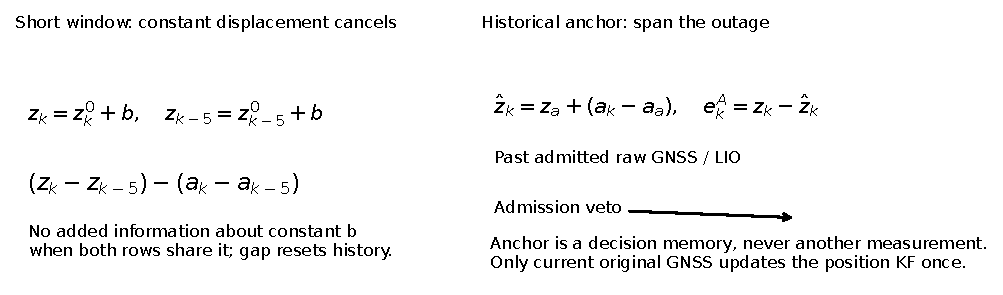
\includegraphics[width=.98\textwidth]{figures/A_anchor_concept.pdf}
\caption{Admission memory. A constant displacement cancels when both endpoints of the five-second window carry it. A historical raw GNSS/LIO correspondence can span the outage. It provides a veto, never another independent position measurement. The right-hand relation also carries historical receiver error and relative-LIO drift.}\label{fig:concept}
\end{figure*}

\subsection{Short Window and Historical Anchor}
Let $a_k$ be the antenna position derived from the independent local LIO cache and fixed alignment. The five-second short window forms
\begin{align}
 d_{ik} &=(z_k-z_i)-(a_k-a_i),\\
 s_{ik} &= d_{ik,xy}^{\top}C_{ik}^{-1}d_{ik,xy},\label{eq:short}\\
 C_{ik} &=R_{k,xy}+R_{i,xy}+(q_t\Delta t+q_d\Delta D)I,
\end{align}
where $q_t=q_d=0.001$ in the corresponding units and $\Delta D$ is accumulated local travel. A constant injected displacement cancels in~\eqref{eq:short} when both rows share it; onset and termination can still be visible. Gaps exceeding 1.5 s clear this window.

The historical anchor stores raw position $z_a$, local antenna position $a_a$, covariance, time and ID. Promotion requires an admitted NORMAL observation, verified local health, short score at most four and acceptable nominal NIS, continuously qualified for five seconds. An actual GNSS gap exceeding two seconds activates the retained anchor. During recovery,
\begin{align}
 e_k^A &= z_k-\{z_a+(a_k-a_a)\},\label{eq:anchor}\\
 s_k^A &= (e_{k,xy}^A)^\top C_{ak}^{-1}e_{k,xy}^A.
\end{align}
The fixed covariance-growth multiplier is one. An available healthy anchor with $s_k^A>4$ vetoes the current admission and resets qualification. Promotion is frozen while the anchor remains active or the motion manager overrides the mature recovery rule. These scores are engineering normalizations, not calibrated independent chi-square evidence.

The manager isolates inconsistent motion or outage returns, applies a two-second minimum wait and requires two seconds of qualifying motion. Since the short window spans five seconds, clean actual admission is commonly seven seconds, not the nominal two-second duration. In RECOVERING, covariance protection begins at 15 and relaxes quadratically over 15 s; renewed inconsistency can isolate again. After 60 s unresolved isolation is reported without inventing a successful admission. The availability shadow retains mature fixed recovery when local evidence is unavailable. Cache endpoints must each have at least 100 effective points and mean absolute plane residual at most 0.2 m; failure triggers logged fallback, not proof of receiver correctness.

\subsection{What an Anchor Can and Cannot Distinguish}
Let $p^{\rm ref}_{\rm ant}$ denote the offline reference antenna position, $\epsilon^G_k=z_k-p^{\rm ref}_{\rm ant,k}$ and
\begin{equation}
 \epsilon^L_{ak}=(a_k-a_a)-(p^{\rm ref}_{\rm ant,k}-p^{\rm ref}_{\rm ant,a}).
\end{equation}
Then~\eqref{eq:anchor} decomposes exactly as
\begin{equation}
 e_k^A=\epsilon^G_k-\epsilon^G_a-\epsilon^L_{ak}.\label{eq:decomp}
\end{equation}
This identity supports offline interpretation only. Relative-LIO drift can either mask an injected offset or make a clean receiver inconsistent. The online manager sees scores, age and local diagnostics, not these reference-derived error terms. A high point count and low fitting residual do not certify an accurate accumulated displacement.

\section{Experimental Protocol and Evidence Audit}
\subsection{Data Roles and Shared Interfaces}
Six i2Nav-Robot routes~\cite{i2nav} remain: building00 (development), parking00 (retrospective), building01 (earlier independent transfer), street00/playground00/building02 (later frozen tests). All are now seen. A second building00 cache is same-bag sensitivity. The shared fixed pipeline uses AT128, ADIS16465 increments and F9P single-point positions; S10 requires no frontend or estimator rerun.

Policies share cache, rows, initialization, Q/R and calibration. Resolved identities and source dispatch verify P/no-anchor differ only by the anchor switch. One predetermined reference state initializes fixed local-to-NED alignment; subsequent reference states remain offline. Evaluation uses common reference/IMU/cache support. Per-route GPS weeks and the 18-s GPS--UTC offset are resolved; increments are not rates. street00's duplicate first reference timestamp uses stable first-row retention without raw changes.

building00/street00/playground00/building02 use navigation-grade GNSS/INS references; parking00/building01 use MM/INS references with shared AT128 map matching. Reference independence from every sensing/error source is not established. Known initialization and alignment also condition receiver-error labels. These are comparative replay experiments, not absolute-origin recovery demonstrations.

\subsection{Fixed Perturbations, Policies and Endpoints}
All original natural runs and seven GNSS perturbation categories remain archived: single/clustered jumps, 30/60-s deletions with unchanged return, 30-s deletions followed by 3/10-m persistent offsets, and a ramp. We independently recompute the 3-m, 10-m and clean 30-s-return cases without changing event identities. The three fixed outage onsets are 150/450/750 s from initialization, with N/E/NE offset directions. Each persistent offset lasts 90 s after return; its norm is 3 or 10 m, with NE normalized. Ninety displaced IDs and thirty deleted IDs are checked per event; other raw IDs, times and receiver standard deviations are unchanged.

Nineteen fixed strategies are retained, including LIO-only B2, direct position KF B3, wide NIS100 B4, Huber2.5 B5, mature Fixed2 B6, strict NIS gates 11.3448667301/16.266236/30, Clock2/5/10/15/30/60/90, P and its no-motion/no-anchor/no-decay ablations. Clock labels denote qualification durations; obtaining the five-second window can add delay. NIS100 is not the strict gate. Aliases may coincide on a case and are not independent algorithms. No-decay disables covariance relaxation/protection within the inherited manager; it is not promoted to a retuned winning method.

For a complete 10-Hz post-return grid, horizontal RMSE is computed separately over 90 s and then averaged equally across the three events. It is not the RMSE of pooled event samples. The 180-s extension is secondary. All expected timestamps are retained; missing coverage cannot be repaired by selecting successful intersections. Actual admission is the first logged \texttt{accepted=true} update after the first physically present return, with 180-s right censoring (C180). Measurement-time admission and conservative cache-availability bounds remain separate; neither is live end-to-end latency. Biased-return delay is distinct from delay after a clean return.

Joint qualification Q requires complete coverage, every clean measurement-time delay at most 15 s, and natural-route RMSE below the best B4/B5/B6 natural error plus $\max(2\%,0.05\,\mathrm{m})$. Unqualified long waits stay in raw comparisons. Accepted injected IDs measure controlled exposure, not field fault probability. Statistical significance from treating correlated epochs or sequential events as independent is not claimed.

\subsection{Independent Audits and Injection Cancellation}
The audit traces original IDs and raw/cache/config/run hashes; independent full-grid metrics match archives. Offline receiver errors use the original antenna lever arm and reference-attitude interpolation. A displacement can reduce existing error rather than create a 3-m absolute error. Among 270 primary rows, cancellation counts are building00 \val{building00cancel}, parking00 \val{parking00cancel}, building01 \val{building01cancel}, street00 \val{street00cancel}, playground00 \val{playground00cancel}, building02 \val{building02cancel}; repeat \val{building00_repeatcancel} separately. All policies' accepted/rejected error distributions and the same 10-m audit are supplied.

street00 has no 3-m cancellation, removing that explanation but not reference/initialization limits. Paired diagnostics distinguish direct veto, qualification delay, correction and prior-state separation, checking~\eqref{eq:decomp} offline. One unsupported route-tail query failed and is retained; scoping diagnosis to fixed event windows/used anchor epochs changed no metric or estimator.

\begin{table*}[t]
\caption{Six routes, all already seen in this post-hoc analysis. 3-m post90 event-macro errors (m); P natural RMSE / inherited cap (m); maximum actual clean delay $T_c$ (s). Lower raw controls remain visible even outside Q.}\label{tab:routes}
\centering\small\setlength{\tabcolsep}{5pt}
\begin{tabular}{lrrrrrcc}\toprule
Route & P & No anchor & Strict NIS0 & Clock90 & P natural / cap & $T_c$ & Q\\\midrule
building00 & \val{building00P90} & \val{building00N90} & \val{building00NIS90} & \val{building00Clock90} & \val{building00natural}/\val{building00cap} & \val{building00clean} & \val{building00qualified}\\
parking00 & \val{parking00P90} & \val{parking00N90} & \val{parking00NIS90} & \val{parking00Clock90} & \val{parking00natural}/\val{parking00cap} & \val{parking00clean} & \val{parking00qualified}\\
building01 & \val{building01P90} & \val{building01N90} & \val{building01NIS90} & \val{building01Clock90} & \val{building01natural}/\val{building01cap} & \val{building01clean} & \val{building01qualified}\\
street00 & \val{street00P90} & \val{street00N90} & \val{street00NIS90} & \val{street00Clock90} & \val{street00natural}/\val{street00cap} & \val{street00clean} & \val{street00qualified}\\
playground00 & \val{playground00P90} & \val{playground00N90} & \val{playground00NIS90} & \val{playground00Clock90} & \val{playground00natural}/\val{playground00cap} & \val{playground00clean} & \val{playground00qualified}\\
building02 & \val{building02P90} & \val{building02N90} & \val{building02NIS90} & \val{building02Clock90} & \val{building02natural}/\val{building02cap} & \val{building02clean} & \val{building02qualified}\\
\bottomrule\end{tabular}

\end{table*}

\section{Results and Discussion}
\subsection{Local Gain against Complete Strong Controls}
Table~\ref{tab:street} retains every policy. On street00, P's 3-m post90 macro is \val{Pstreet90} m versus no-anchor \val{Pwithoutanchorstreet90} m, a \val{streetImprovement}\% reduction. Strict NIS gives \val{NIS0street90} m and Huber \val{B5street90} m. The best standard raw control is Clock60 at \val{Clock60street90} m, despite its \val{Clock60clean}-s clean delay. Clock90 waits beyond the finite injection, accepts none of its rows and has \val{Clock90street90}-m error at \val{Clock90clean}-s clean delay. Their exclusion from Q does not hide their raw results.

\begin{table}[t]
\caption{street00 controlled 3-m results, all 19 fixed policies. $R_{90}/R_{180}$: event-macro horizontal RMSE (m). $T_c$: maximum actual clean admission (s); C180 is censored. $n_b$: accepted injected rows out of 270. Q combines natural cost, clean service and coverage.}\label{tab:street}
\centering\small\setlength{\tabcolsep}{3pt}
\begin{tabular}{lrrrrc}\toprule
Policy & $R_{90}$ & $R_{180}$ & $T_c$ & $n_b$ & Q\\\midrule
LIO only & \val{B2street90} & \val{B2street180} & \val{B2clean} & \val{B2accepted} & \val{B2qualified}\\
Direct KF & \val{B3street90} & \val{B3street180} & \val{B3clean} & \val{B3accepted} & \val{B3qualified}\\
NIS100 & \val{B4street90} & \val{B4street180} & \val{B4clean} & \val{B4accepted} & \val{B4qualified}\\
Huber2.5 & \val{B5street90} & \val{B5street180} & \val{B5clean} & \val{B5accepted} & \val{B5qualified}\\
Fixed2 & \val{B6street90} & \val{B6street180} & \val{B6clean} & \val{B6accepted} & \val{B6qualified}\\
NIS11.3449 & \val{NIS0street90} & \val{NIS0street180} & \val{NIS0clean} & \val{NIS0accepted} & \val{NIS0qualified}\\
NIS16.2662 & \val{NIS1street90} & \val{NIS1street180} & \val{NIS1clean} & \val{NIS1accepted} & \val{NIS1qualified}\\
NIS30 & \val{NIS2street90} & \val{NIS2street180} & \val{NIS2clean} & \val{NIS2accepted} & \val{NIS2qualified}\\
Clock2 & \val{Clock2street90} & \val{Clock2street180} & \val{Clock2clean} & \val{Clock2accepted} & \val{Clock2qualified}\\
Clock5 & \val{Clock5street90} & \val{Clock5street180} & \val{Clock5clean} & \val{Clock5accepted} & \val{Clock5qualified}\\
Clock10 & \val{Clock10street90} & \val{Clock10street180} & \val{Clock10clean} & \val{Clock10accepted} & \val{Clock10qualified}\\
Clock15 & \val{Clock15street90} & \val{Clock15street180} & \val{Clock15clean} & \val{Clock15accepted} & \val{Clock15qualified}\\
Clock30 & \val{Clock30street90} & \val{Clock30street180} & \val{Clock30clean} & \val{Clock30accepted} & \val{Clock30qualified}\\
Clock60 & \val{Clock60street90} & \val{Clock60street180} & \val{Clock60clean} & \val{Clock60accepted} & \val{Clock60qualified}\\
Clock90 & \val{Clock90street90} & \val{Clock90street180} & \val{Clock90clean} & \val{Clock90accepted} & \val{Clock90qualified}\\
P-r03 & \val{Pstreet90} & \val{Pstreet180} & \val{Pclean} & \val{Paccepted} & \val{Pqualified}\\
No motion & \val{Pwithoutmotionstreet90} & \val{Pwithoutmotionstreet180} & \val{Pwithoutmotionclean} & \val{Pwithoutmotionaccepted} & \val{Pwithoutmotionqualified}\\
No anchor & \val{Pwithoutanchorstreet90} & \val{Pwithoutanchorstreet180} & \val{Pwithoutanchorclean} & \val{Pwithoutanchoraccepted} & \val{Pwithoutanchorqualified}\\
No decay & \val{Pwithoutdecaystreet90} & \val{Pwithoutdecaystreet180} & \val{Pwithoutdecayclean} & \val{Pwithoutdecayaccepted} & \val{Pwithoutdecayqualified}\\
\bottomrule\end{tabular}

\end{table}

P satisfies natural \val{streetPNatural} m against the \val{streetPCap}-m cap and seven-second clean admission in every event. Clock2 has similar nominal qualification and the same clean delay, but lacks the historical veto. The single-switch no-anchor contrast is the sharper attribution control because it retains the rest of P's machinery. Importantly, no-decay gives \val{Pwithoutdecaystreet90} m with the same controlled exposure and clean delay. P does not beat all nineteen variants; covariance decay is not necessary for this observed benefit.

\begin{figure*}[t]
\centering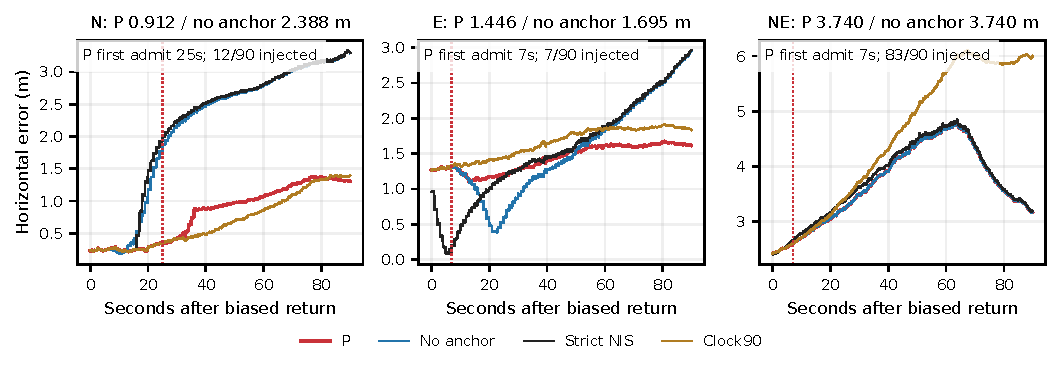
\includegraphics[width=.98\textwidth]{figures/B_street_all_events.pdf}
\caption{Every fixed street00 3-m event. Curves are actual horizontal errors on the full post90 grid. Labels show P's first actual biased-return admission and accepted injected IDs. Two events improve; NE has no additional anchor rejection and is nearly neutral. Delaying biased observations is not the clean-service endpoint.}\label{fig:street}
\end{figure*}

\subsection{Event-Level Admission Attribution}
Table~\ref{tab:events} and Fig.~\ref{fig:street} prevent a route mean from hiding the third event. At Event0, P/no-anchor pre-fault positions agree exactly (\val{streetPrior0} m). P first admits at \val{event0delay} s and accepts \val{event0accept}/90 injected rows, versus seven-second no-anchor admission. It rejects \val{event0extra} additional IDs that no-anchor accepts; actual strict NIS accepts \val{event0nisextra} of these. Of \val{streetVeto0} direct anchor vetoes, \val{streetShort0} occur with an available short-window score at most four. P briefly admits biased observations, so this is not perfect discrimination. Nevertheless, the matched state, switch and per-ID decisions locate a concrete additional-memory effect: post90 RMSE is \val{event0P} rather than \val{event0N} m.

\begin{table}[t]
\caption{All street00 3-m events. $R$: post90 horizontal RMSE (m); $T_b$: P's actual biased-return admission (s); $n_P$: P accepted injected IDs /90. Extra: IDs rejected by P but accepted by no-anchor. NIS-extra: those also accepted by the actual strict NIS policy.}\label{tab:events}
\centering\small\setlength{\tabcolsep}{2pt}
\begin{tabular}{lrrrrrrr}\toprule
Event & $R_P$ & $R_{NA}$ & $R_{NIS}$ & $T_b$ & $n_P$ & Extra & NIS+\\\midrule
0 (N) & \val{event0P} & \val{event0N} & \val{event0NIS} & \val{event0delay} & \val{event0accept} & \val{event0extra} & \val{event0nisextra}\\
1 (E) & \val{event1P} & \val{event1N} & \val{event1NIS} & \val{event1delay} & \val{event1accept} & \val{event1extra} & \val{event1nisextra}\\
2 (NE) & \val{event2P} & \val{event2N} & \val{event2NIS} & \val{event2delay} & \val{event2accept} & \val{event2extra} & \val{event2nisextra}\\
\bottomrule\end{tabular}

\end{table}

At Event1, P rejects \val{event1extra} additional IDs, all \val{event1nisextra} accepted by strict NIS; its \val{streetVeto1} direct vetoes follow an initially permissive anchor. The error decreases from \val{event1N} to \val{event1P} m. This is supporting evidence with sequential-history dependence: prior positions already differ by \val{streetPrior1} m, so it is not another independently initialized replicate.

At Event2 there are \val{event2extra} additional rejected IDs. P accepts \val{event2accept}/90, and its error differs from no-anchor by only \val{streetNeutralDelta} m. This is residual history, not a third anchor-detection success. The error decomposition shows how local-motion error can reduce an anchor contradiction; it cannot define an online eligibility rule. Across all events, strict NIS accepts \val{NIS0accepted}/270 displaced IDs, versus P \val{Paccepted}/270; this exposure contrast alone is not an accuracy theorem.

\subsection{Why the 10-m Control Matters}
For street00's inherited 10-m case, strict NIS0 and P give \val{street10NIS} and \val{street10P} m, respectively, and both reject all 270 displaced rows. Their near equality is retained rather than converted into a general claim that NIS fails. The 3-m result shows that a displacement can remain below a policy's innovation threshold while crossing its historical-motion score. Short-window cancellation is verified on paired raw differences, but absolute drift and prior receiver error determine whether an anchor actually helps in a particular event.

\begin{figure*}[t]
\centering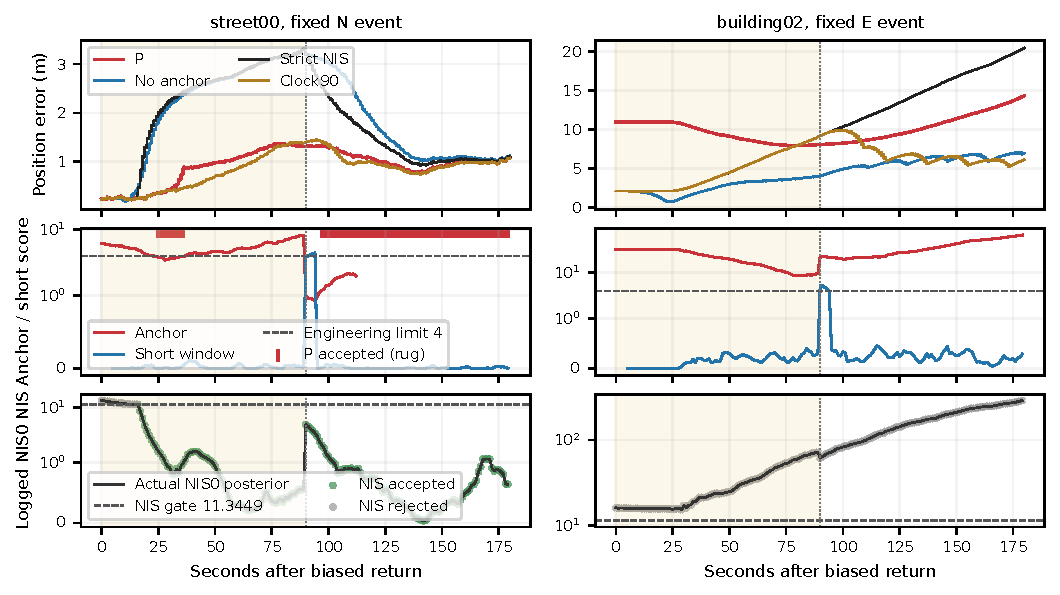
\includegraphics[width=.98\textwidth]{figures/C_fixed_mechanism_timelines.pdf}
\caption{Representative timelines declared before score reconstruction: street00 Event0 (N) and building02 Event1 (E). Top: actual position errors; middle: logged P anchor/short-window scores, engineering limit four and accepted-update rug; bottom: actual strict NIS posterior scores and decisions. Shading denotes the 90-s displaced interval. The negative event already has \val{building02Prior}-m P/no-anchor prior-state separation, so its later divergence is not a fresh isolated anchor effect. Missing scores remain missing.}\label{fig:timeline}
\end{figure*}

\begin{figure*}[t]
\centering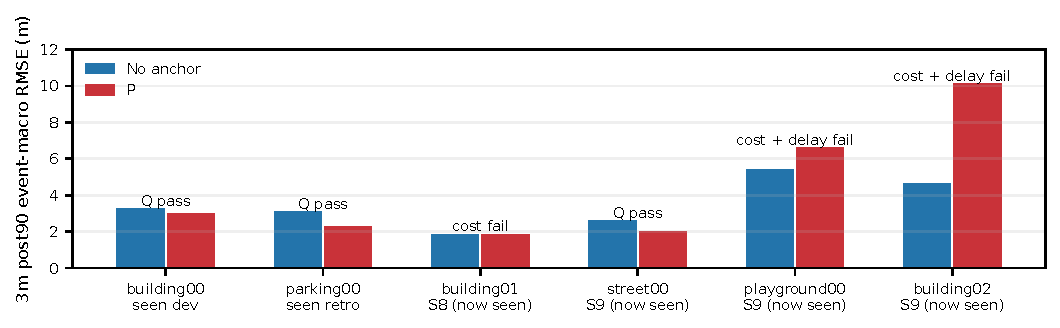
\includegraphics[width=.98\textwidth]{figures/D_all_six_route_contrasts.pdf}
\caption{All six route contrasts and P's original Q status. Opposing signs, cost failures and delay failures are retained. The same-bag repeat is reported separately and does not inflate scene count. No adverse route or event is removed after inspecting accuracy.}\label{fig:routes}
\end{figure*}

\subsection{Counterexamples and Service Failures}
Figure~\ref{fig:routes} and Table~\ref{tab:routes} retain all six route signs. building00 improves against no-anchor, but Clock90 has lower raw error and 95-s clean admission. The second building00 cache yields P/no-anchor \val{repeatP}/\val{repeatPwithoutanchor} m and remains only sensitivity. parking00 improves against no-anchor but strict NIS is lower. building01 has equal P/no-anchor error and fails natural cost. Its large cancellation count also cautions against equating artificial amplitude with absolute receiver error.


playground00 and building02 both worsen against no-anchor and fail natural and clean-service constraints. Their clean delays include 142 s and an event still unadmitted at 180 s. Rejecting all biased rows does not protect against excessive LIO drift. The building02 timeline shows an anchor veto even as the short-window check becomes permissive, but prior-state carryover is already substantial. Offline relative-LIO error reaches \val{building02Motion} m over that biased event; the next event is also adverse.

Clean controls provide less confounded failure evidence. In playground00 clean Event1 and building02 clean Event2, P/no-anchor prior positions agree exactly (\val{playCleanPrior}/\val{buildCleanPrior} m), yet the anchor vetoes all ninety return rows; 85 have a qualifying short score. Relative-LIO error reaches \val{playCleanMotion}/\val{buildCleanMotion} m offline, and P's post90 error penalty is \val{playCleanPenalty}/\val{buildCleanPenalty} m. All relevant point/residual health flags pass. Thus currently logged health and anchor availability do not certify an accurate historical extrapolation. A truth-free condition separating beneficial and harmful vetoes has not been validated.


\subsection{Scope of the Scientific Claim}
The supported claim is a descriptive street00 3-m macro advantage against standard controls under unchanged costs, with direct single-switch evidence in Event0. There is no general operating condition, independent confirmation or novelty proof. Sequential events share history; time/direction are confounded. The stronger no-decay variant and adverse routes bound this result.

Separate archived native KF-GINS natural errors on street00/playground00/building02 are \val{street00nativehorizontal_rmse_m}/\val{playground00nativehorizontal_rmse_m}/\val{building02nativehorizontal_rmse_m} m (playground00 coverage \val{playground00nativecoverage}), lower than P. These are real independent GNSS/INS comparators, not same-injection results or P-gain denominators. Earlier 10-m joint failures and R1's no-additional-gain conclusion are unchanged. Reference/GNSS correlations, shared AT128 mapping on two routes, controlled single-reference initialization and the unresolved \val{frontendRepeat}-m RMS frontend repeat difference limit generalization. Cache replay and availability clocks do not demonstrate live realtime latency or natural multipath detection.

\section{Conclusion}
Unchanged historical admission memory improves two street00 3-m events under the inherited service/cost constraints; the third is neutral. Matched decisions locate additional memory beyond NIS and short windows. No-decay is stronger and other routes fail. Confirmation requires unseen data, preregistered hypotheses and an online applicability condition; this post-hoc case supplies none.

\section*{Evidence Availability and Review Disclosure}
Audited CSVs, all policy decisions, figure points, source/input/run hashes and failures accompany the preserved S10 branch. No new amplitude experiment or method revision was performed. Codex (GPT-6) assisted tooling, checks, figures and drafting throughout. Human authors must verify metadata, claims, originality and venue disclosure. This is a tutor-review manuscript, not a formal submission.

\bibliographystyle{IEEEtran}
\bibliography{references}
\end{document}
